%%% DOCUMENT CONFIGURATION %%%

\documentclass[
	letterpaper, % Paper size, use either a4paper or letterpaper
	10pt, % Default font size, can also use 11pt or 12pt, although this is not recommended
	unnumberedsections, % Comment to enable section numbering
	twoside, % Two side traditional mode where headers and footers change between odd and even pages, comment this option to make them fixed
]{LTJournalArticle}

\addbibresource{sample.bib} % BibLaTeX bibliography file

\setcounter{page}{1} % The page number of the first page, set this to a higher number if the article is to be part of an issue or larger work

\usepackage{amsmath}

%%% TITLE SECTION %%%

\title{Leveraging Neural Networks for Efficient Obstacle\\Avoidance and Racing an Autonomous Car}
% Article title, use manual lines breaks (\\) to beautify the layout

% Authors are listed in a comma-separated list with superscript numbers indicating affiliations
% \thanks{} is used for any text that should be placed in a footnote on the first page, such as the corresponding author's email, journal acceptance dates, a copyright/license notice, keywords, etc

\author{Yanxiang Zhang, Chaarvi Goel, Siddharth H. Nair, Francesco Borrelli
\thanks{\;Y. Zhang and C. Goel are with the Department of Electrical Engineering and Computer Sciences, S. H. Nair is with the Department of Mechanical Engineering, University of California, Berkeley, Berkeley, CA 94701, USA \texttt{\{joshzhang, chaarvigoel, siddharth\_nair, fborrelli\}@berkeley.edu}}}

\date{}    % This prevents a bug idk
\begin{document}
\maketitle % Output the title section

%%% ARTICLE CONTENTS %%%

\textbf{\small\textit{Abstract}---In this paper we present a novel neural network model capable of predicting a large number of output dimensions from minimal input data. This research addresses the challenges in autonomous car technology, particularly in high-speed environments with limited visibility. The model, developed using PyTorch, demonstrates exceptional efficiency in path planning, reducing problem-solving time by a factor of 100 while maintaining over 95\% accuracy. This achievement sets a new benchmark for the application of neural networks in high-speed, real-time scenarios. The effectiveness of the proposed strategy is demonstrated by experimental results on the Berkeley Autonomous Race Car (BARC) platform.}

\section{I. INTRODUCTION}

Autonomous cars, obstacle avoidance, and efficient racing are at the forefront of modern technological advancements. The development of autonomous vehicles has been a significant milestone in the field of artificial intelligence and machine learning. This research area has evolved rapidly, with key milestones including the integration of neural networks for enhanced decision-making and the implementation of sophisticated algorithms for dynamic obstacle avoidance.

The motivation behind this research lies in the utilization of neural networks to predict essential variables for obstacle avoidance offline. This approach significantly minimizes the computation required for path planning when encountering new obstacles, thereby maximizing the race car's speed in terms of problem-solving time and time to reach a goal. The importance of this research is underscored by the growing demand for efficient and safe autonomous vehicles in various sectors, including transportation and logistics.

In the realm of machine learning and autonomous vehicles, several approaches have been explored to tackle the challenges of obstacle avoidance and efficient path planning. However, many of these methods still grapple with the limitations of real-time data processing and computational efficiency. Our research identifies a gap in the current machine learning landscape, where there is a need for models that can predict complex variables with high accuracy and minimal computational demand. This gap is particularly evident in scenarios with limited visibility and high-speed requirements, common in racing environments.

The primary objective of this paper is to demonstrate the feasibility of using a neural network model to accurately predict a large number of output dimensions from a relatively small number of input dimensions. Our focus is on a model that can process inputs consisting of the car’s position, velocity in the x and y directions, and obstacles detected within a limited field of vision. The goal is to train this model to predict 500 binary variables that are crucial for efficient and effective path planning in real-time racing scenarios.

Our contribution to the field of machine learning and autonomous vehicles is significant. We have developed and trained a PyTorch model capable of performing binary classification of variables used in solving a convex optimization problem for path planning. This model stands out for its ability to reduce problem-solving time by a factor of 100 while maintaining an accuracy rate of over 95 percent. This achievement not only proves the feasibility of racing an autonomous car with efficient, on-the-fly obstacle avoidance but also sets a new benchmark in the application of neural networks in high-speed autonomous vehicle operations.

The novel aspect of our research lies in the unique application of neural networks to a highly specialized domain of autonomous racing. Our approach differs from existing methods by focusing on the prediction of a large number of output variables from limited input data, a challenge that has not been extensively explored in current research. This innovation opens up new possibilities for machine learning in areas where real-time data processing and decision-making are critical.

This paper is organized as follows: In Section II we introduce the problem definition. Section III illustrates our methodology in structuring the neural networks. Section IV illustrates our experimental process and tuning the models. Finally, in Section V we present our results on the BARC. Section VI provides final remarks.

\section{II. PROBLEM DEFINITION}

\quad Consider the following state and input vectors:
\[x = [p_x, p_y, v_x, v_y], \quad u = [a_x, a_y]\]

\noindent where \(Px, Py\) are the vehicle’s position and \(Vx, Vy\) are the vehicle’s velocity on the x and y axes. \(Ax, Ay\) are the vehicle’s acceleration inputs along their respective axes. For the purpose of computation, the vehicle is described by a point mass. For implementation on a physical car, the magnitudes of the variables are constrained by:
\[\left| v_x \right|, \left| v_y \right| \leq \sqrt{0.5} \, \text{m/s}, \quad \left| a_x \right|, \left| a_y \right| \leq 1 \, \text{m/s}^2\]

The vehicle’s navigable environment is modeled by the first and fourth quadrants of a coordinate plane, where the origin is situated at the midpoint of the left “wall”. The environment is bounded by a height h in the y-direction and a width w in the (strictly positive) x-direction. For the purpose of physical implementation, we assume that \(h = 2.5\)m and \(w = 5.0\)m, and that the “goal” state the vehicle must reach from any random starting state is always
\[x_{goal} = [5.0, 0.0, 0.0, 0.0].\]

Within the environment lies a number of rectangular obstacles with random dimensions and positions. Each obstacle is modeled by a pair of tuples:
\[obs_l = (l_x, l_y), \quad obs_s = (s_x, s_y).\]

\(obs_l\) is the coordinates of the obstacle’s lower left-hand corner, and \(obs_s\) is the length of the obstacle along the x and y axes. For the purpose of this experiment, we assume a fixed number of obstacles (five), each with fixed dimensions and positions as shown in Figure 1.

Each instance of the motion planning problem starts at timestep \(t=0\), where the vehicle is given a random starting state. \(Px, Py\) must lie inside the environment’s boundaries and outside any obstacles, and \(Vx = Vy\) = 0.0. For each discrete timestep \(t\) in
\[0 \leq t < t_{end}, \quad \text{where}\; t_{end}\; \text{is when} \quad x[t_{end}] = x_{goal},^\dagger\]

\noindent the vehicle will scan up to a distance \(d\) in four cardinal directions and detect an obstacle if any edge lies within
\[p_x \leq edge \leq p_x \pm d, \quad p_y \leq edge \leq p_y \pm d.\]

For purposes of this experiment, we assume that \(d = 1.25^\dagger\)m and the difference \(\Delta\) between adjacent timesteps \(\Delta = t_1 - t_0 = 0.1^\dagger\)s.

\textit{\(^\dagger\)Side note: we selected 1.25m for \(d\) to simulate a limited range of visibility for obstacle detection. This range could be modeled as a radius; Section IV details an alternative approach that results in a more computationally efficient model. We selected 0.1s for \(\Delta\) to match the vehicle's response time to our input signal at each timestep. \(x[t_{end}] = x_{goal}\) was computed with a tolerance of 0.1 in total magnitude.}

\begin{figure}
	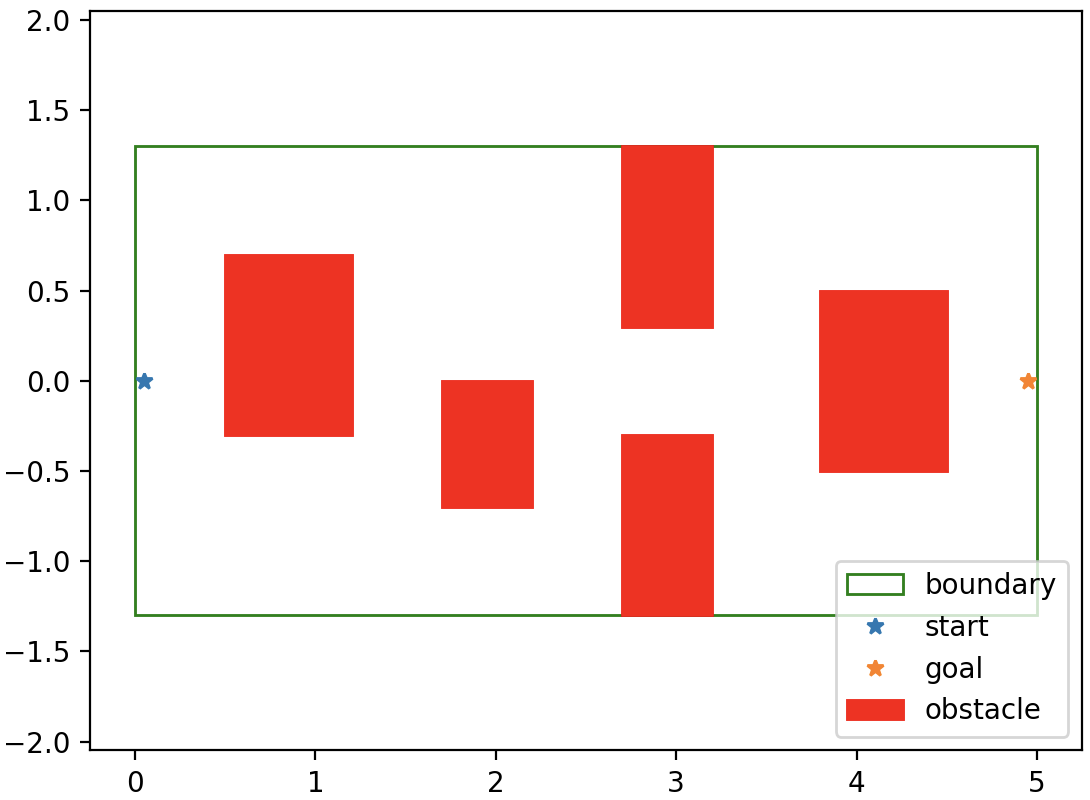
\includegraphics[width=\linewidth]{world.png}
	\caption{Rendering of the vehicle's environment and obstacles.}
\end{figure}

\subsubsection{Motion Planning Problem.} This algorithm constitutes the computational runtime that our neural network seeks to minimize. We structured it as a convex optimization problem in Python using the \texttt{cvxpy} library. The problem is given input Parameters:
\[x,\; x_{goal},\; obs\_lower,\; obs\_size\]

\noindent where the latter two are arrays of \(obs_l\) and \(obs_s\) tuples representing obstacles the vehicle has detected so far. The problem outputs Variables:
\[x_{sol},\; u_{sol},\; b\_l_{sol},\; b\_u_{sol}\]

\noindent which are the optimal state, input, and binary variables for obstacle avoidance that the algorithm solves for. The vehicle's dynamics are modeled by the state matrix \( A \) and input matrix \( B \):
\begin{align*}
    & A = \begin{bmatrix}
        1 & 0 & dt & 0 \\
        0 & 1 & 0 & dt \\
        0 & 0 & 1 & 0  \\
        0 & 0 & 0 & 1
    \end{bmatrix}, \quad
    B = dt \begin{bmatrix}
        0.5 \cdot dt & 0 \\
        0 & 0.5 \cdot dt \\
        1 & 0 \\
        0 & 1
    \end{bmatrix} \\
    & \text{where} \quad x[t+\Delta] = Ax[t] + Bu[t].
\end{align*}

Obstacle avoidance constraints are implemented using the Big-M method. For each obstacle, \(b\_l_{sol}\) and \(b\_u_{sol}\) are introduced, with the matrix \(M\) given by:
\[M = \begin{bmatrix}
2 \cdot max(a_x) & 0 \\
0 & 2 \cdot max(a_y)
\end{bmatrix}\]

For each obstacle \(i\), binary constraints are given by:
\begin{align*}
    & x[t+\Delta] \leq obs\_lower^{(i)} + M \times b\_l_{sol}^{(i)}[t], \\
    & x[t+\Delta] \geq obs\_upper^{(i)} - M \times b\_u_{sol}^{(i)}[t], \\
    & b\_l_{sol}^{(i)}[0, k] + b\_l_{sol}^{(i)}[1, k] + b\_u_{sol}^{(i)}[0, k] + b\_u_{sol}^{(i)}[1, k] < 4
\end{align*}

\noindent where \(obs\_upper\) is an array of tuples representing the upper right-hand corners of obstacles, formed by the element-wise addition of tuples in \(obs\_lower\) and \(obs\_size\). The last constraint ensures that the vehicle's position is not bounded by all four walls of an obstacle.

Cost constraints are modeled by the state matrix \(Q\), input matrix \(R\), and horizon \(N\) (the number of timesteps \(\Delta\) to calculate starting from current time \(t\):
\[Q = 100 \cdot I_{(4\times4)}, \quad R = 50 \cdot I_{(2\times2)}, \quad N = 25\]

\noindent where the cost function \(J\) is a weighted sum of the deviation from the goal state and the control inputs:
\[\sum_{k=0}^{N-1} \left( \| Q (x[t] - x_{goal}) \| + \| R u[t] \| \right) + p \| x[N] - x_{goal} \|\]

\noindent where \(p\) is a large penalty on the terminal state \(x[N]\) to encourage approaching \(x_{goal}\).
The problem is thus formulated as minimizing \(J\) subject to the above constraints for (\(t = 0, 1, \ldots, N-1\)). This definition allows for an efficient computation of the optimal trajectory, avoiding obstacles while minimizing the cost function.

\section{III. PROPOSED METHODS}

Aenean feugiat pellentesque venenatis. Sed faucibus tristique tortor vel ultrices. Donec consequat tellus sapien. Nam bibendum urna mauris, eget sagittis justo gravida vel. Mauris nisi lacus, malesuada sit amet neque ut, venenatis tempor orci. Curabitur feugiat sagittis molestie. Duis euismod arcu vitae quam scelerisque facilisis. Praesent volutpat eleifend tortor, in malesuada dui egestas id. Donec finibus ac risus sed pellentesque. Donec malesuada non magna nec feugiat. Mauris eget nibh nec orci congue porttitor vitae eu erat. Sed commodo ipsum ipsum, in elementum neque gravida euismod. Cras mi lacus, pulvinar ut sapien ut, rutrum sagittis dui. Donec non est a metus varius finibus. Pellentesque rutrum pellentesque ligula, vitae accumsan nulla hendrerit ut.

Aenean porttitor eros non pharetra congue. Proin in odio in dolor luctus auctor ac et mi. Etiam euismod mi sed lectus fringilla pretium. Phasellus tristique maximus lectus et sodales. Mauris feugiat ligula quis semper luctus. Nam sit amet felis sed leo fermentum aliquet. Mauris arcu dui, posuere id sem eget, cursus pulvinar mi. Donec nec lacus non lectus fermentum scelerisque et at nibh. Sed tristique, metus ac vestibulum porta, tortor lectus placerat lorem, et convallis tellus dolor eget ante. Pellentesque dui ligula, hendrerit a purus et, volutpat tempor lectus. Mauris nec purus nec mauris rhoncus pellentesque. Quisque quis diam sed est lacinia congue. Donec magna est, hendrerit sed metus vel, accumsan rutrum nibh.

Orci varius natoque penatibus et magnis dis parturient montes, nascetur ridiculus mus. Etiam cursus lectus purus, tempus iaculis quam dictum tristique. Nam interdum sapien nec tempor mattis. Quisque id sapien nisi. Mauris vehicula ornare eros vel efficitur. Nulla consectetur, turpis quis fringilla tincidunt, mi neque iaculis lectus, vel commodo elit odio non ex. Duis facilisis, purus ac viverra iaculis, turpis lectus ultrices ante, ac vestibulum ligula magna in libero. Etiam tristique maximus lacinia. Vestibulum hendrerit, lacus malesuada laoreet blandit, sapien velit sollicitudin nunc, eu porttitor urna ligula at lorem. Aliquam faucibus eros in fermentum venenatis. Fusce consectetur congue pellentesque. Suspendisse at nisi sit amet est porttitor cursus. Cras placerat faucibus nunc, a laoreet justo dignissim sit amet.

Orci varius natoque penatibus et magnis dis parturient montes, nascetur ridiculus mus. Etiam cursus lectus purus, tempus iaculis quam dictum tristique. Nam interdum sapien nec tempor mattis. Quisque id sapien nisi. Mauris vehicula ornare eros vel efficitur. Nulla consectetur, turpis quis fringilla tincidunt, mi neque iaculis lectus, vel commodo elit odio non ex. Duis facilisis, purus ac viverra iaculis, turpis lectus ultrices ante, ac vestibulum ligula magna in libero. Etiam tristique maximus lacinia. Vestibulum hendrerit, lacus malesuada laoreet blandit, sapien velit sollicitudin nunc, eu porttitor urna ligula at lorem. Aliquam faucibus eros in fermentum venenatis. Fusce consectetur congue pellentesque. Suspendisse at nisi sit amet est porttitor cursus. Cras placerat faucibus nunc, a laoreet justo dignissim sit amet.

%------------------------------------------------

\section{IV. RESULTS \& ANALYSIS}

\begin{figure}
	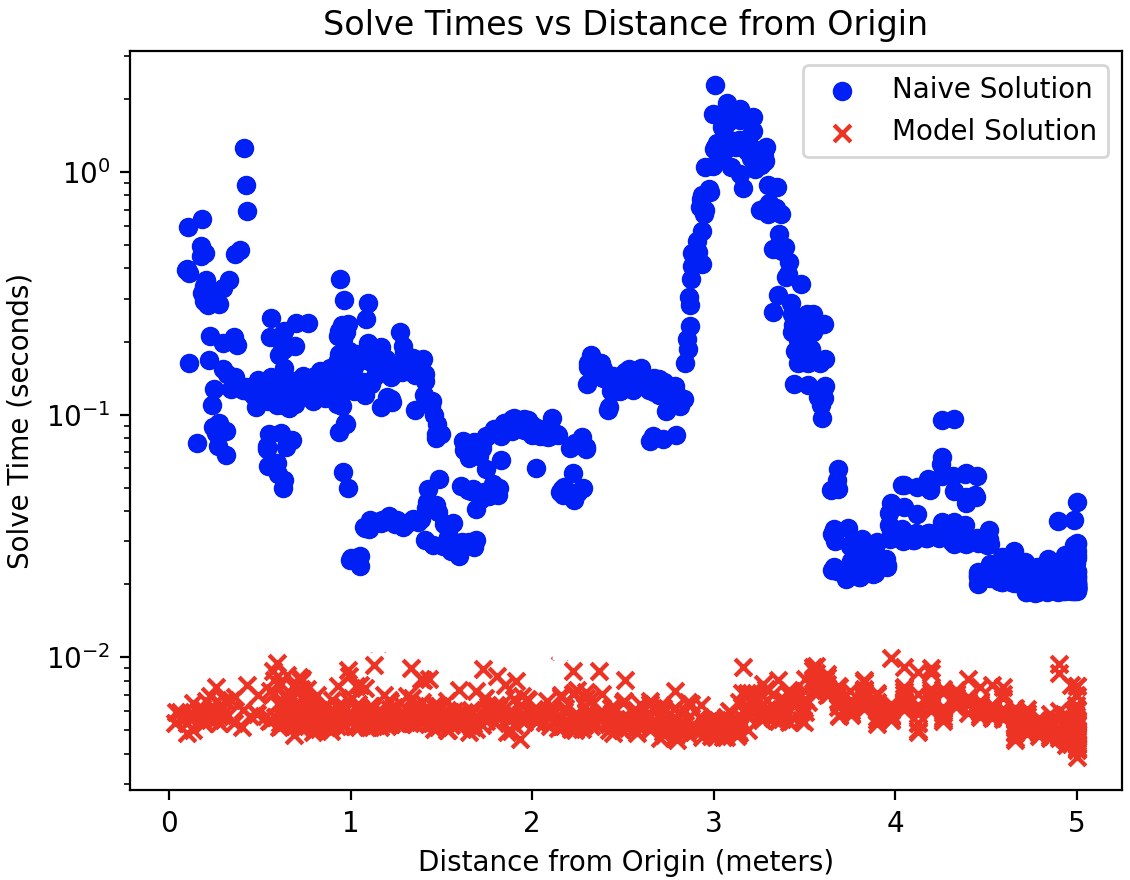
\includegraphics[width=\linewidth]{graph.png}
	\caption{Solve times vs distance from origin for both methods.}
\end{figure}

\begin{table}
    \caption{Comparison of metrics between naive and model methods.}
    \centering
    \begin{tabular}{l r r}
        \toprule
        Solve Time Metric & Naive Soln. & Model Soln. \\
        \midrule
        Minimum & 0.01844  & 0.003887 \\
        Median  & 0.08775  & 0.005787 \\
        Maximum & 2.2856   & 0.009929 \\
        Average & 0.1868   & 0.005978 \\
        Standard Deviation & 0.3277 & 0.000948 \\
        \bottomrule
    \end{tabular}
\end{table}

Suspendisse potenti. Vivamus suscipit dapibus metus. Proin auctor iaculis ex, id fermentum lectus dapibus tristique. Nullam maximus eros eget leo pretium dapibus. Nunc in auctor erat, id interdum risus. Suspendisse aliquet vehicula accumsan. In vestibulum efficitur dictum. Sed ultrices, libero nec fringilla feugiat, elit massa auctor ligula, vehicula tempor ligula felis in lectus. Suspendisse sem dui, pharetra ut sodales eu, suscipit sit amet felis. Donec pretium viverra ante, ac pulvinar eros. Suspendisse gravida consectetur urna. Pellentesque vitae leo porta, imperdiet eros eget, posuere sem. Praesent eget leo efficitur odio bibendum condimentum sit amet vel ex. Nunc maximus quam orci, quis pulvinar nibh eleifend ac. Quisque consequat lacus magna, eu posuere tellus iaculis ac. Sed vitae tortor tincidunt ante sagittis iaculis.

Nullam mollis tellus lorem, sed congue ipsum euismod a. Donec pulvinar neque sed ligula ornare sodales. Nulla sagittis vel lectus nec laoreet. Nulla volutpat malesuada turpis at ultricies. Ut luctus velit odio, sagittis volutpat erat aliquet vel. Donec ac neque eget neque volutpat mollis. Vestibulum viverra ligula et sapien bibendum, vel vulputate ex euismod. Curabitur nec velit velit. Aliquam vulputate lorem elit, id tempus nisl finibus sit amet. Curabitur ex turpis, consequat at lectus id, imperdiet molestie augue. Curabitur eu eros molestie purus commodo hendrerit. Quisque auctor ipsum nec mauris malesuada, non fringilla nibh viverra. Quisque gravida, metus quis semper pulvinar, dolor nisl suscipit leo, vestibulum volutpat ante justo ultrices diam. Sed id facilisis turpis, et aliquet eros.

\section{V. CONCLUSION}

Duis venenatis eget lectus a aliquet. Integer vulputate ante suscipit felis feugiat rutrum. Aliquam eget dolor eu augue elementum ornare. Nulla fringilla interdum volutpat. Sed tincidunt, neque quis imperdiet hendrerit, turpis sapien ornare justo, ac blandit felis sem quis diam. Proin luctus urna sit amet felis tincidunt, sed congue nunc pellentesque. Ut faucibus a magna faucibus finibus. Etiam id mi euismod, auctor nisi eget, pretium metus. Proin tincidunt interdum mi non interdum. Donec semper luctus dolor at elementum. Aenean eu congue tortor, sed hendrerit magna. Quisque a dolor ante. Mauris semper id urna id gravida. Vestibulum mi tortor, finibus eu felis in, vehicula aliquam mi.

Aliquam arcu turpis, ultrices sed luctus ac, vehicula id metus. Morbi eu feugiat velit, et tempus augue. Proin ac mattis tortor. Donec tincidunt, ante rhoncus luctus semper, arcu lorem lobortis justo, nec convallis ante quam quis lectus. Aenean tincidunt sodales massa, et hendrerit tellus mattis ac. Sed non pretium nibh. 

Donec cursus maximus luctus. Vivamus lobortis eros et massa porta porttitor. Nam vitae suscipit mi. Pellentesque ex tellus, iaculis vel libero at, cursus pretium sapien. Curabitur accumsan velit sit amet nulla lobortis, ut pretium ex aliquam. Proin eget volutpat orci. Morbi eu aliquet turpis. Vivamus molestie urna quis tempor tristique. Proin hendrerit sem nec tempor sollicitudin.

%%% REFERENCES %%%

\printbibliography % Output the bibliography
\end{document}